\documentclass[
    ../../Software_Engineering_Summary.tex,
]
{subfiles}

\externaldocument[ext:]{../../Software_Engineering_Summary.tex}
% Set Graphics Path, so pictures load correctly
\graphicspath{{../../}}

\begin{document}
\section{Design Patterns}
A design pattern describes 
\begin{itemize}
    \item a problem that reoccurs regularly in the domain
    \item the core of a solution to this problem, such that one can reuse the solution in other contexts (might not be exactly the same)
\end{itemize}

\begin{defbox}
    [Template Method Pattern]
    Implements an algorithm in a manner that allows adaptation to different implementations.

    \begin{itemize}
        \item Define skeleton algorithm, but defer implementation of some concrete parts to subclasses
        \item Often used in frameworks and APIs
    \end{itemize}

    Some benefits:
    \begin{itemize}
        \item Separation of variant and invariant parts
        \item Avoidance of unnecessary code duplication
        \item Control of subclass extensions
    \end{itemize}
    
\end{defbox}

\begin{defbox}
    [Design Pattern Template]
    \begin{enumerate}
        \item 
        \begin{itemize}
            \item Name: Short mnemonic to extend the design vocabulary
            \item Intent: Goals and reasons why to use the pattern
        \end{itemize}
        \hrulefill
        \item 
        \begin{itemize}
            \item Motivation: States problem situation
            \item Applicability: Context in which the pattern can be used
        \end{itemize}
        \hrulefill
        \item 
        \begin{itemize}
            \item Structure: Static structure of the pattern (UML Class diagram)
            \item Participants: Which classes are involved 
            \item Collaborations: How the classes interact
            \item Implementation: How to implement the pattern
        \end{itemize}
        \hrulefill
        \item 
        \begin{itemize}
            \item Consequences: Gains and trade-offs
        \end{itemize}
        \hrulefill
        \item 
        \begin{itemize}
            \item Known Uses: Examples of using the pattern
            \item Related Patterns: References to and discussion of related patterns
        \end{itemize}
    \end{enumerate}
\end{defbox}

\begin{minipage}
    [t]{0.5\textwidth}
    \centering
    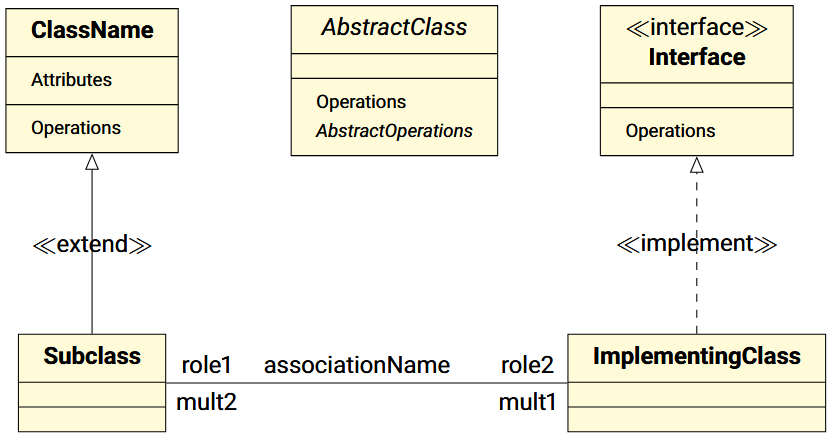
\includegraphics[width=\textwidth]{Pics/09/DesignPatternUMLClassDiagram.png}
\end{minipage}
\hfill
\begin{minipage}
    [t]{0.5\textwidth}
    \centering
    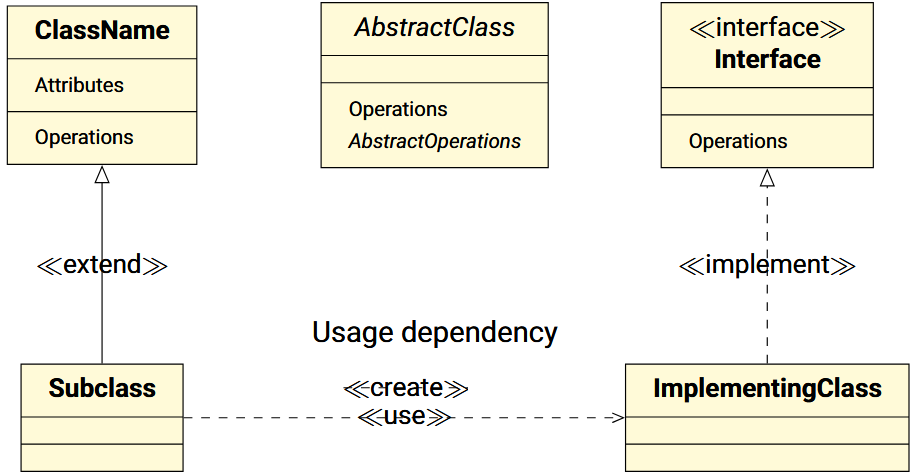
\includegraphics[width=\textwidth]{Pics/09/DesignPatternUMLClassDiagram1.png}
\end{minipage}

\subsection{Subject - Observer Pattern}

The subject - observer pattern utilizes
Object-Oriented Analysis and Design (OOAD).
OOAD organizes a problem by breaking it down into managable subtasks \rightarrow Objects are responsible for subtasks. Collaboration might be required for complex problems.

\defc{Advantages:}
\begin{itemize}
    \item Easy to understand, implement, understand, maintain and reuse objects - Divide and Conquer approach possible
    \item Flexible combinations for different problems possible
\end{itemize}

\defc{Disadvantages:}
\begin{itemize}
    \item Behaviour is distributed across objects \rightarrow Lack of clarity of design
    \item Any state change might affect others
\end{itemize}

Hereby the communication of the objects is desirable to be done with low coupling, as change in one object should not necessarily result in change in another. This way the objects can be reused in different context.

\subsubsection{Subject - Observer Pattern: Pull Mode}
Subject is an object with state changes that are independent of the observers. The observers get information from the subject and react accordingly.

\begin{minipage}
    [t]{0.5\textwidth}
    \centering
    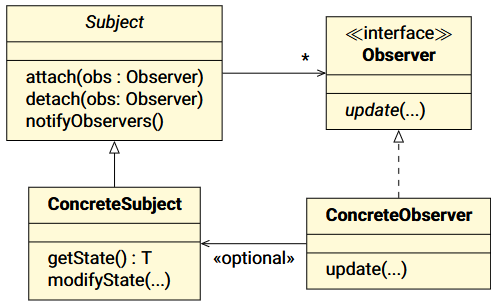
\includegraphics[width=0.95\textwidth]{Pics/09/ObserverPattern.png}
\end{minipage}
\hfill
\begin{minipage}
    [t]{0.5\textwidth}
    \centering
    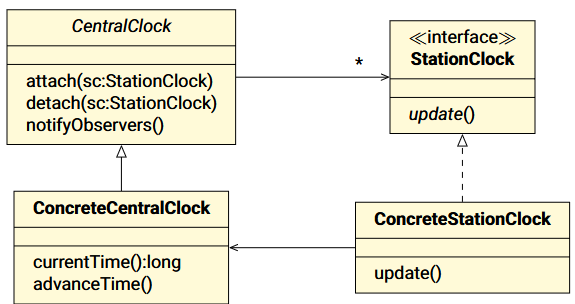
\includegraphics[width=\textwidth]{Pics/09/ObserverPatternExample.png}
\end{minipage}

\begin{itemize}
    \item Subject should not need to know details about its observers
    \item Identity and number of observers not predetermined or fixed
    \item New observers can be added dynamically
\end{itemize}

\begin{defbox}
    [Observer Pattern - Advantages]
    \begin{itemize}
        \item Abstract coupling between \defc{subject} and \defc{observer}
        \item Support for broadcast communication 
        \begin{itemize}
            \item Sender does not know the type of the receiver
        \end{itemize}
    \end{itemize}
\end{defbox}

\begin{defbox}
    [Observer Pattern - Disadvantages]
    \begin{itemize}
        \item Danger of update cascades from observers to their dependant objects
        \item Update sent to all observers - might not be interesting to all observers
        \item No change details - Observers need to find out what has changed
        \item Uniform interface for all observer updates - Subject cannot send optional parameters to observers
    \end{itemize}
\end{defbox}

\begin{codebox}
    [Example: Car Inventory]
    \begin{lstlisting}[language=Java]
class CarInventoryView implements Observer {
    @Override
    public void update(Subject subject) {
        fillTable((CarInventory) subject);
    }
}\end{lstlisting}
\end{codebox}

\subsubsection{Subject - Observer Pattern: Push Mode}
Instead of just passing the current state of the subject to every observer additionally also provides the change in the state. Observers can then handle their actions according to the change and do not necessarily need to access the state of the subject

\begin{codebox}
    [Example: Car Inventory]
    \begin{lstlisting}[language=Java]
class CarInventoryView implements Observer {
    @Override
    public void update(Subject subject, Change change) {
        if(change.getKind() == Change.CarDeletion) {
            deleteRowForCar(change.getCar());
        } else(change.getKind() == Change.CarAddition) {
            ...                    
        }
    }
}\end{lstlisting}
\end{codebox}

\subsubsection{Subject - Observer Pattern: Interest Mode}

When registering observer to subject, specify what kind of updates the observer is interested in. This way the observer doesn't have ot check whether the update is of interest or not, and can skip right to handling it. This, of course, means that the subject has to handle more as it can't just send out a pure update notification.

For example: Java Action Listeners, Mouse Listeners etc.

\subsection{Factory Method}

In a framework that needs to be able to present multi-format documents like PDF, HTML, Word etc. the framework should be able to do so, while offering common functionality. (open, close, save, print, etc.) 

This can essentially be done by letting these different classes implement a common interface, but leave instantation of a specific class to the factory.

\begin{codebox}
    [Example: Factory Method]
    \begin{minipage}
        [t]{0.5\textwidth}
        Abstract:
	\begin{lstlisting}[language=Java]
public abstract class Document {
    public void open();
    public void close();
    ...
}

public abstract class Application {
    private List<Document> docs = new ArrayList<>();

    public void newDocument() {
        Document doc = createDocument();
        docs.add(doc);
        doc.open();
    }
    public abstract Document createDocument();
}\end{lstlisting}
\end{minipage}
\hfill
\begin{minipage}
    [t]{0.5\textwidth}
    Concrete:
    \begin{lstlisting}[language=Java]
public class TextDocument extends Document {
    ...
}

public class MyApplication extends Application {
    public Document createDocument() {
        return new TextDocument();
    }
}
\end{lstlisting}
\end{minipage}
\end{codebox}

The creator can also be implemented concretely, providing a reasonable default implementation.

\begin{minipage}
    [t]{0.5\textwidth}
    \centering
    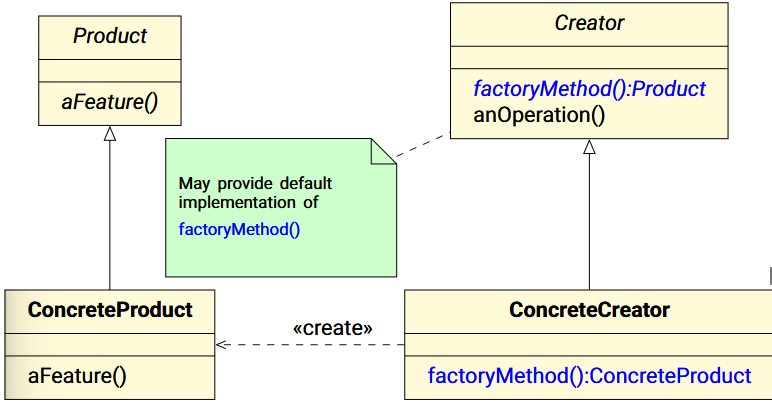
\includegraphics[width=\textwidth]{Pics/09/FactoryMethod.png}
\end{minipage}
\hfill
\begin{minipage}
    [t]{0.5\textwidth}
    \centering
    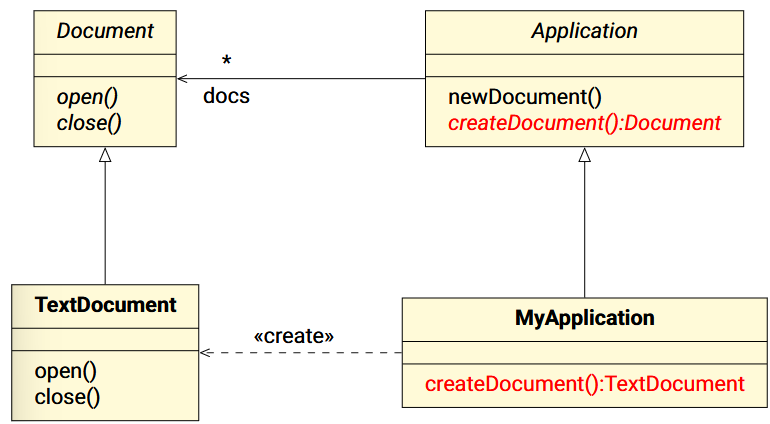
\includegraphics[width=\textwidth]{Pics/09/FactoryMethodExample.png}
\end{minipage}

\begin{defbox}
    [Factory Method - Consequences]
    \begin{itemize}
        \item Client application code only knows product  interface \rightarrow Works for any ConcreteProduct
        \item Product provides a hook for subclasses \rightarrow Extended version of object via hook
    \end{itemize}
\end{defbox}

\subsection{Abstract Factory}

Abstract Factories provide a system to create a family of related classes that implement common interfaces. 

For example, taking a search engine that needs to search for a query in multiple databases of different formats: 

\begin{figure}
    [htp]
    \centering
    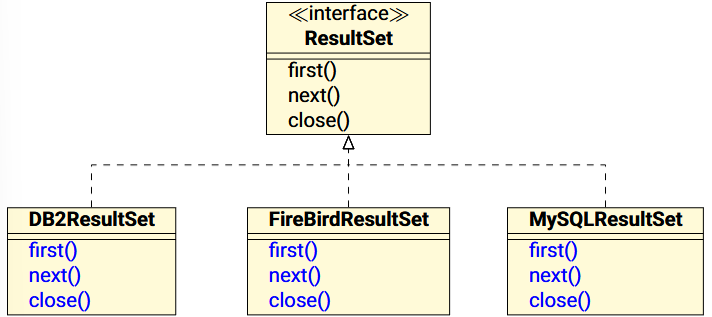
\includegraphics[width = 0.5\textwidth]{Pics/09/AbstractFactory_DatabaseExample.png}
\end{figure}

This creates a problem of that this usually needs to still have concrete implementations of the subclasses as the class hierarchy might differ and the interacting code might be different.
Additionally, this method requires that the format is specified at the time of creation, which is undesirable. 

The solution is to have an interface, the abstract factory, that is used to instantiate the concrete factories, which in turn can then be used to create the concrete classes.

\begin{minipage}
    [t]{0.5\textwidth}
    \centering
    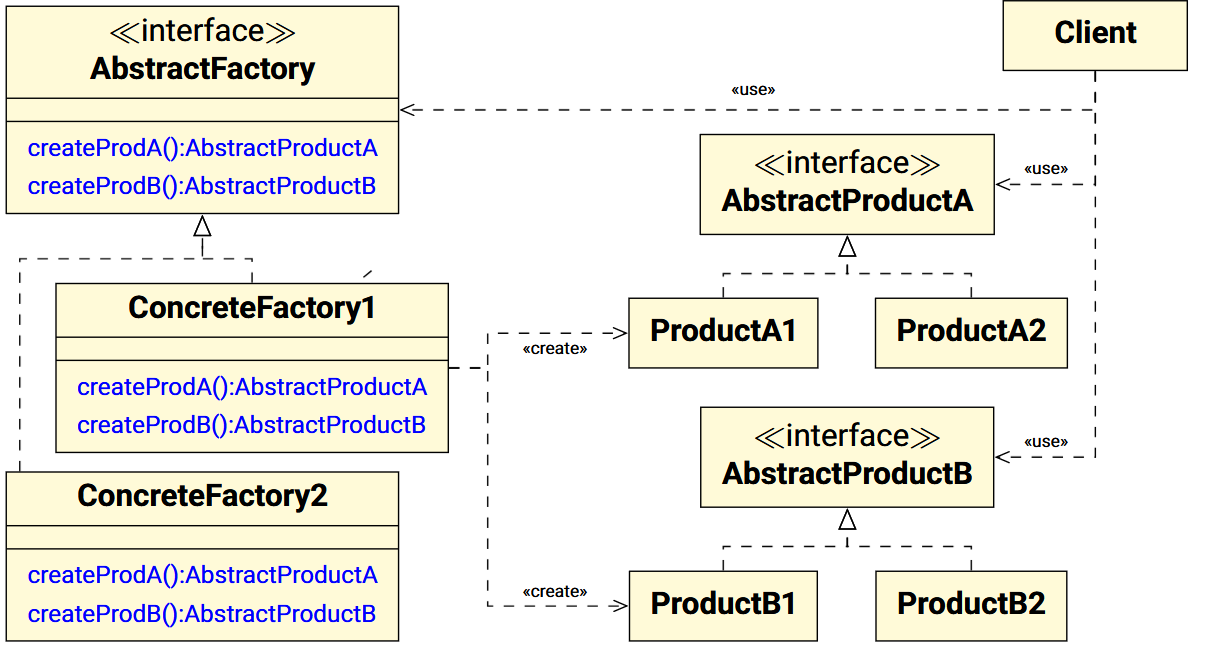
\includegraphics[width=\textwidth]{Pics/09/AbstractFactory.png}
\end{minipage}
\hfill
\begin{minipage}
    [t]{0.5\textwidth}
    \centering
    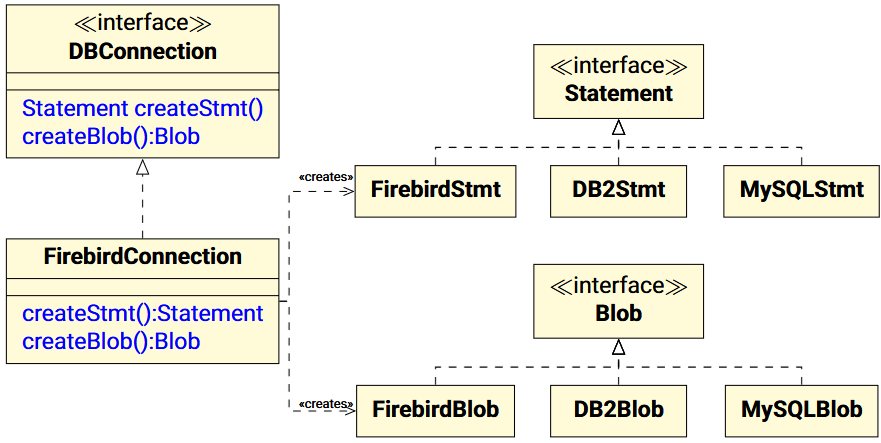
\includegraphics[width=\textwidth]{Pics/09/AbstractFactoryExample.png}
\end{minipage}

\begin{defbox}
    [Abstract Factory - Advantages]
    \begin{itemize}
        \item Abstracts concrete products - Client is unaware of the concrete product they're using
        \item Changing formats/families is easy
        \item Consistency among products
    \end{itemize}
\end{defbox}

\begin{defbox}
    [Abstract Factory - Disadvantages]
    \begin{itemize}
        \item Adding unforseen additional products is expensive - Abstract family and all its subclasses need to be changed
        \item Object creation follown non-standard pattern - Factory instead of constructor
    \end{itemize}
\end{defbox}

\subsection{Factory Method vs. Abstract Factory}

\begin{defbox*}

    \begin{center}
	\begin{tabular}{|c|c c|}
        \hline
        & Factory Method & Abstract Factory\\
        \hline
        \hline
        Product & Single & Family\\
        \hline
        Product declaration & Client & Startup\\
        \hline
        Product exchange & Concrete Product & Abstract Product\\
        \hline 
        Creation & Local (Creator) & Selection of Factory\\
        \hline
    \end{tabular}
    \end{center}
\end{defbox*}
\end{document}